\textbf{BERT}  
With the transformer architecture proposed, a lot of transformer related models saw emergence the years thereafter. Such model was the Bidirectional Encoder Representations from Transformers (BERT) utilizing only the encoders from the transformer architecutre, and OpenAIs GPT utilizing only the decoder structure. This model was yet another huge jump forward in the field of NLP in machine learning\cite{devlin_bert_2019}.

A noteable problem with purely transformer encoder-based models, which BERT is, was that training on word prediction and similar could be problematic. Since the encoder structure employ the self-attention mechanism, it allows it to see the target token. This is the reason that OpenAIs GPT model opted for a decoder structure, a purely left-to-right model structure, as it allowed them to perform next work prediction without the model being able to see the word it was to predict due to the masked self attention.

The training process for BERT allows it to use an encoder based implementation where each work during training has a chance to be either: masked, replaced or retainted as-is; they denote this as "Masked Language Model" pre-training objective. The training process is then for the model to predict the "masked" word. This novelization of the training process allows the model to be bidirectional and use the encoders from the transformer architecture, and thus have a better understanding of the context of the words in a sentence - both left \textit{and} right - which they claim is crucial for models to do tasks such as question answering. The representations that BERT learn could also be used for downstream tasks such as classification, questioning and answering, sentiment analysis et cetera.

The Masked Language Model training objective is utilized in other models as well as other domains including audio; as an example, W2V-BERT utilizes it\cite{chung_w2v-bert_2021}.

\begin{figure}
    \centering
    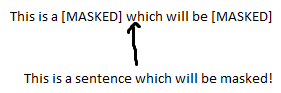
\includegraphics[width=0.75\textwidth]{figures/MLM.png}
    \caption{Masked Language Model Pretraining PLACEHOLDER}
    \label{fig:mlm}
\end{figure}

BERT proved to be an incredibly capable model outperforming in many different tasks proving it to be a very versatile model. The model was also the first to be able to outperform humans in the Stanford Question Answering Dataset (SQuAD) benchmark\cite{rajpurkar2016squad100000questionsmachine}.

\begin{figure}
    \centering
    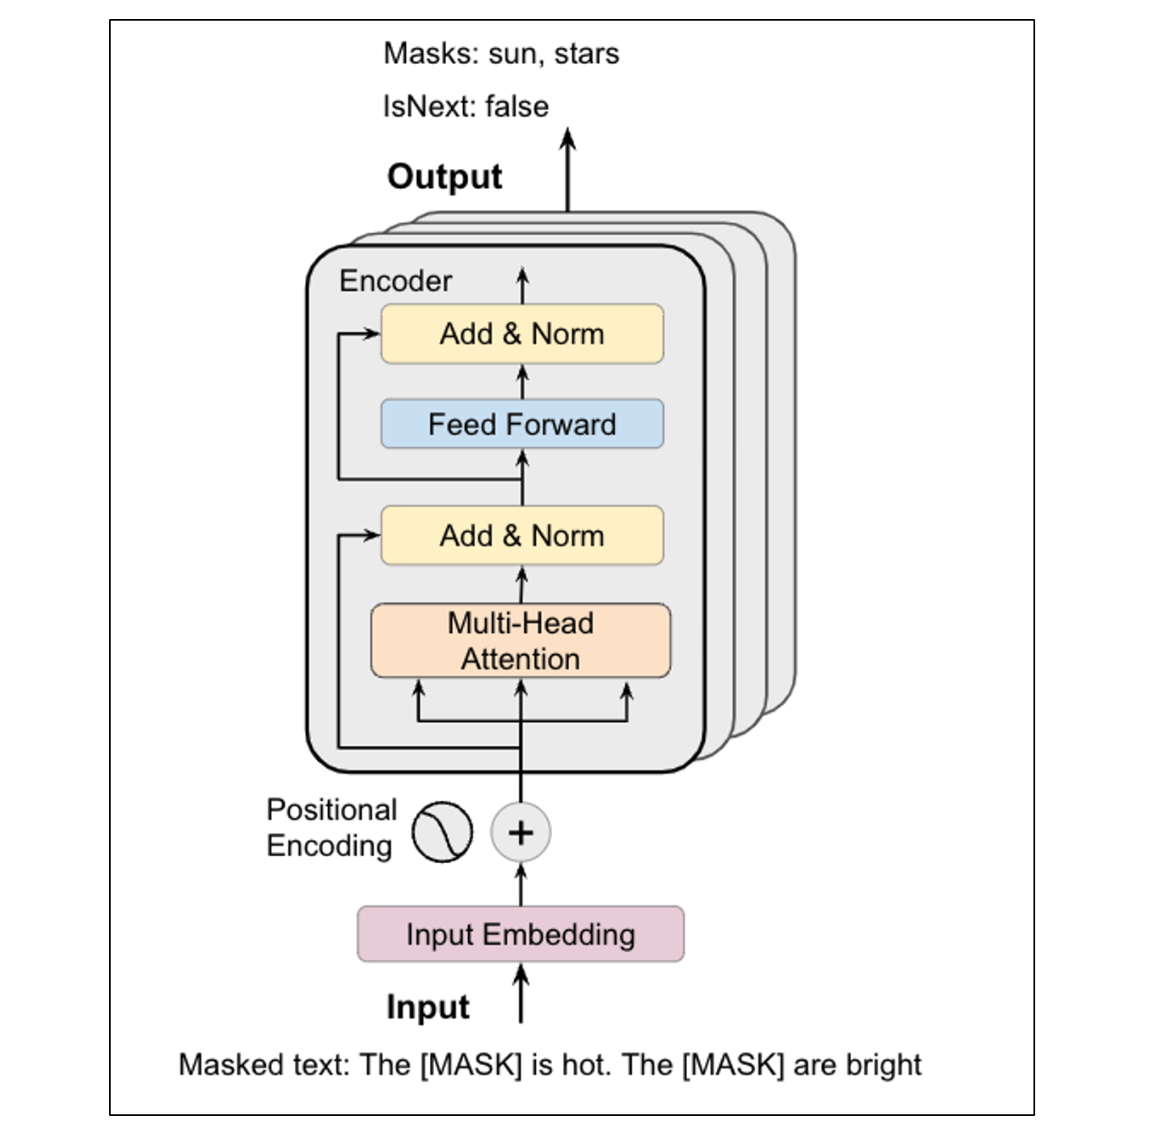
\includegraphics[width=0.5\textwidth]{figures/BERT.png}
    \caption{BERT model architecture here PLACEDHOLDER}
    \label{fig:bert}
\end{figure}